\documentclass{beamer}

\mode<presentation>
{
  \usetheme{CambridgeUS}      % or try Darmstadt, Madrid, ...
  \usecolortheme{default} % or try albatross, beaver, crane, ...
  \usefonttheme{default}  % or try serif, structurebold, ...
  \setbeamertemplate{navigation symbols}{}
  \setbeamertemplate{caption}[numbered]
} 

\usepackage[english]{babel}
\usepackage[utf8x]{inputenc}
\usepackage{listings}
\usepackage[ampersand]{easylist}



\definecolor{KTI_green}{RGB}{150, 189, 13}
\definecolor{TU_red}{RGB}{255, 55, 81}
\definecolor{faint_gray}{RGB}{180, 180, 180}

\definecolor{syntax_green}{rgb}{0,0.6,0}
\definecolor{syntax_gray}{rgb}{0.9, 0.9, 0.9}
\definecolor{syntax_mauve}{rgb}{0.58,0,0.82}

\lstset{ 
  backgroundcolor=\color{syntax_gray},  % choose the background color
  basicstyle=\scriptsize\ttfamily,        		% size of fonts used for the code
  breaklines=false,                		% automatic line breaking only at whitespace
  captionpos=b,                    		% sets the caption-position to bottom
  commentstyle=\color{syntax_green},    % comment style
  escapeinside={\%*}{*)},          		% if you want to add LaTeX within your code
  keywordstyle=\color{blue},       		% keyword style
  stringstyle=\color{syntax_mauve},     % string literal style
  columns=fullflexible,
  frame=single,
  framesep=0.5cm,
  framexleftmargin=0.5cm,
  xleftmargin=0.5cm,
  framexrightmargin=0.5cm,
  xrightmargin=0.5cm,
  frame=tb,                 
    numbers=left,                    
    numbersep=15pt,  
  }
  
  
\newcommand{\logopython}{\raggedleft 
\includegraphics[height=0.5cm]{logo_python}\hspace{0.1cm}\\\raggedright}
\newcommand{\logopythonbottom}{\raggedleft\vspace{-0.8cm}
\includegraphics[height=0.5cm]{logo_python}\hspace*{0.05cm}\\\raggedright}

\title[BSP04 - Geburtstage]{Geburtstage}
\author{Dickbauer Y., Moser P., Perner M.}
\institute{PS Computergestützte Modellierung, WS 2016/17}
%\date{Date of Presentation}

\begin{document}

\begin{frame}
  \titlepage
\end{frame}

% Uncomment these lines for an automatically generated outline.
\begin{frame}{Outline}
  \tableofcontents
\end{frame}

\section{Aufgabenstellung}
\begin{frame}{Aufgabenstellung}
In einem Seminar sitzen x Teilnehmer. Ermitteln Sie n¨aherungsweise mittels Simulation
die Wahrscheinlichkeit, dass zwei Teilnehmer am selben Tag Geburtstag haben.

\begin{itemize}
  \item Eingabe: Anzahl an Teilnehmer, Anzahl an Simulationsdurchläufen
  \item Durchschnittliche Wahrscheinlichkeit, dass zwei Teilnehmer am selben Tag
Geburtstag haben.
  \item Output optional: Ausgabe der Geburtstage und Markierung der Tage, wo mehr als
eine Person Geburtstag hat.
\end{itemize}

\end{frame}

\section{Flow Chart}
\begin{frame}{Flow Chart}
	\centering
  	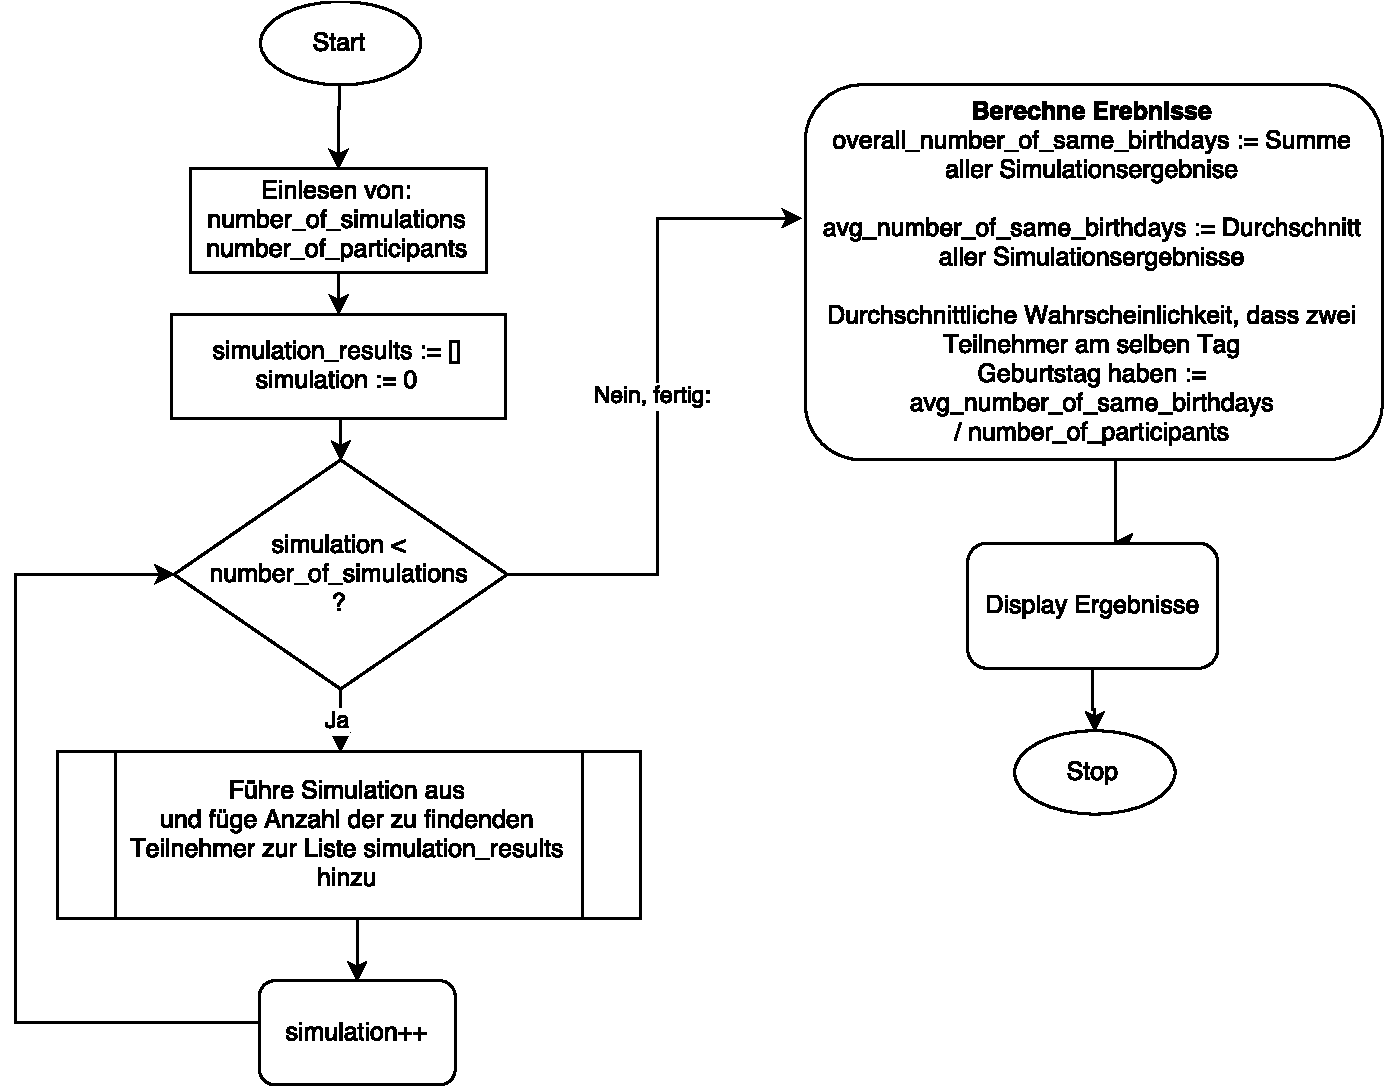
\includegraphics[scale=0.4]{BSP04_Flow_Chart_1.pdf}
\end{frame}
\section{Flow Chart}
\begin{frame}{Flow Chart - Ein Simulationsdurchgang}
	\centering
  	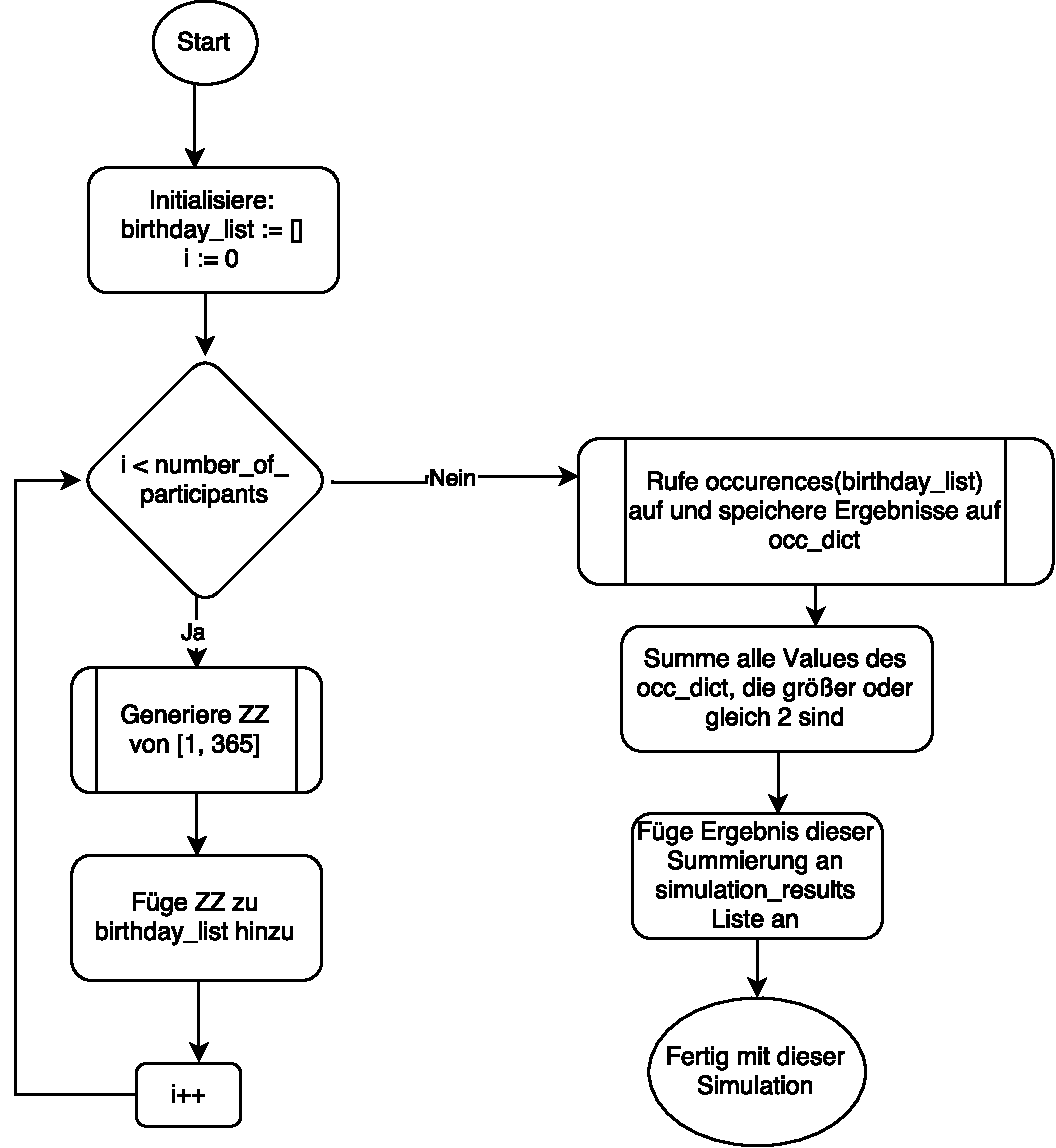
\includegraphics[scale=0.4]{BSP04_Flow_Chart_2.pdf}
\end{frame}

\section{Programmcode}
\subsection{Main Funktion}
\begin{frame}[fragile]{Main Funktion - Programmeinstieg}
  \begin{lstlisting}[language=python]
def main():
    #user input:
    number_of_simulations, number_of_participants = user_input((
        ('Number of simulations', int, 100),
        ('Number of participants', int, 40)), DEBUG)
        
    simulation_results = []
    for simulation in range(number_of_simulations):
        # generate a list of birthdays - with length of participants
        birthday_list = []
        for i in range(number_of_participants):
            birthday_list.append( int(random_number_from_interval(0, DAYS_IN_A_YEAR))+1 )
        # count the same candidates:
        occ_dict = occurrences(birthday_list)
        assert sum(occ_dict.values()) == number_of_participants
        number_of_same_values = sum([value if value >= 2 else 0 for key, value in occ_dict.items()])
        simulation_results.append(number_of_same_values)
        
        # output only if option enabled:
        if OPTION:
        	# print those where there are more than two... see source
    
\end{lstlisting}
\logopythonbottom
\end{frame}

\begin{frame}[fragile]{Main Funktion - Programmeinstieg}
  \begin{lstlisting}[language=python]
    # result of all simulations
    overall_number_of_same_birthdays = sum(simulation_results)
    avg_number_of_same_birthdays = overall_number_of_same_birthdays /
    							   number_of_simulations
    simulation_result_p = avg_number_of_same_birthdays /
    					  number_of_participants
    
    print('Ergebnisse aller {0}/{0} Simulationen:'.format(number_of_simulations))
    print('Durchschnittlich haben {} von {} Personen am gleichen Tag Geburtstag.'.format(
        avg_number_of_same_birthdays, number_of_participants))
    print('WSKL ueber alle Simulationen: p={}%'.format(simulation_result_p * 100))
\end{lstlisting}
\logopythonbottom
\end{frame}

\subsection{Verwendete Funktionen}
\begin{frame}[fragile]{Funktion random\_number\_from\_interval(..)}
  \begin{itemize}
    \item Diese Funktion verlangt zwei Eingabeparameter \textit{lower} und \textit{upper}
    \item Gibt eine (pseudo)Zufallszahl (\textit{float}) im Intervall  [\textit{lower}, \textit{upper}) zurück 
    \item \textit{random.random()} ist eine Funktion der Python Standardbibliothek, welche ein Zufallszahl (\textit{float}) im Intervall [\textit{lower}, \textit{upper}) zurück gibt
    \item Mersenne Twister Methode wird als Generator der ZZ verwendet\footnote[frame] {\scriptsize\url{https://docs.python.org/3.5/library/random.html}} \footnote[frame] {\scriptsize\url{https://en.wikipedia.org/wiki/Mersenne_Twister}}
  \end{itemize}
  \begin{lstlisting}[language=python]
def random_number_from_interval(lower, upper):
    val = random.random()
    return lower + (upper -lower) * val
\end{lstlisting}
\logopythonbottom
\end{frame}	
\begin{frame}[fragile]{Funktion user\_input(input\_vars, [use\_defaults])}
  \begin{itemize}
  	\item Diese Funktion verlang vom User die geforderten Eingabeparameter und gibt diese als von der Programmiererin gewünschten Datentyp wieder zurück
    \item Funktion verlangt als ersten Eingabeparameter die Liste \textit{input\_vars}
    \item Falls \textit{use\_defaults == True} wird der User nicht nach Eingabe gefragt (Dient zum Testen)
    \item Diese Liste besteht wiederrum aus Listen mit je Länge = 3:
    \begin{itemize}
    	\item 0: Text, welcher dem User ausgegeben wird
    	\item 1: Datentyp (int/float/str)
    	\item 2: Default value: Dieser Wert wird zurueckgegeben, falls \textit{use\_defaults == True}
    \end{itemize}
  \end{itemize}
  \begin{lstlisting}[language=python]
x, y = user_input((
    ('Geben Sie einen X Wert ein', int, 10),
    ('Geben Sie einen Y Wert ein', int,  5), False):
  \end{lstlisting}
  \logopythonbottom
\end{frame}	
\begin{frame}[fragile]{Funktion occurences(input\_list)}
  \begin{itemize}
    \item Diese Funktion verlangt eine Liste voller Zahlen als Eingabeparameter \textit{input\_list}
    \item Diese Liste wird durchsucht auf alle vorkommenden Zahlen und zählt mit, wie oft welche Zahl in der Liste enthalten ist
    \item Zurückgegeben wird ein \textit{dictionary}, welches jeweils die Zahl als \textit{key} und die Anzahl dieser keys in der Eingabeliste als \textit{value}
    \item Eingabeliste [1,2,3] gibt zurück: \{1: 1, 2: 1, 3: 1\}
    \item Eingabeliste [1,1,2] gibt zurück: \{1: 2, 2: 1\}
  \end{itemize}
  Code:
  \begin{lstlisting}[language=python]
def occurrences(input_list):
    occ_dict = {}
    for elem in input_list:
        if elem in occ_dict:
            occ_dict[elem] += 1
        else:
            occ_dict[elem] = 1
    return occ_dict
  \end{lstlisting}
\logopythonbottom
\end{frame}

\section{Beispiel}
\begin{frame}[fragile]{Beispiel anhand fixer Zufallszahlen}
\begin{itemize}
	\item number\_of\_simulations := 2
	\item number\_of\_participants := 10
\end{itemize}
\begin{easylist}
\ListProperties(Hide=100, Hang=true, Progressive=3ex, Style*= ,
Style2*=$\bullet$ ,Style3*=$\circ$ ,Style4*=\tiny$\blacksquare$ )
& Simulationsdurchgang 0:
&& Geburtstage := \{1, 10, 20, 50, 10, 20, 40, 12, 40, 365\}
&& Ergebnis: 6 (2x10, 2x20, 2x40)
& Simulationsdurchgang 1:
&& Geburtstage := \{2, 10, 77, 40, 15, 20, 77, 12, 40, 365\}
&& Ergebnis: 4 (2x40, 2x77)
\vspace{0.5cm}
& Im Durchschnitt haben 5 Personen am gleichen Tag Geburtstag $\frac{6+4}{2} = 5.$
& Das sind 50\% der Teilnehmer $\frac{6+4}{2*10}$ oder $\frac{5}{10}$
\end{easylist}
\end{frame}

\begin{frame}[fragile]{Anhang: Modifikation des Source Codes um Demo Beispiel zu erhalten}
  \begin{lstlisting}[language=python]
  # Aendere random_number_from_interval() in lib.py wie folgt:
ZZ = [1, 10, 20, 50, 10, 20, 40, 12, 40, 365,
      2, 10, 77, 40, 15, 20, 77, 12, 40, 365]
i = -1
def random_number_from_interval(lower, upper):
    global i
    i += 1
    return ZZ[i]-1
  \end{lstlisting}
\logopythonbottom
\end{frame}
\end{document}
